\documentclass[a4paper,12pt,twoside]{report}

% ====== Encodage & langue ======
\usepackage[utf8]{inputenc}
\usepackage[T1]{fontenc}
\usepackage[french]{babel}

% ====== Mise en page ======
\usepackage[top=2.8cm, bottom=2.8cm, left=2.2cm, right=2.2cm]{geometry}
\usepackage{setspace}
\onehalfspacing
\usepackage{fancyhdr}
\pagestyle{fancy}
\fancyhf{}
\fancyhead[LE,RO]{\thepage}
\fancyhead[LO]{\leftmark}
\fancyhead[RE]{\rightmark}
\renewcommand{\headrulewidth}{0.3pt}
\renewcommand{\footrulewidth}{0pt}
\fancyfoot[L]{ENSIAS - IDSIT 2024/2025}
\fancyfoot[R]{Chaos Engineering}

% ====== Liens ======
\usepackage[hidelinks]{hyperref}

% ====== Graphiques & tableaux ======
\usepackage{graphicx}
\graphicspath{{images/}}
\usepackage{float}
\usepackage{subcaption}
\usepackage{booktabs}
\usepackage{tabularx}
\usepackage{array}
\usepackage{caption}
\captionsetup{font=small, labelfont=bf}

% ====== Code ======
\usepackage{xcolor}
\usepackage{listings}
\lstset{
  basicstyle=\ttfamily\small,
  keywordstyle=\color{blue!70!black},
  stringstyle=\color{red!60!black},
  commentstyle=\color{gray!70!black},
  numbers=left,
  numberstyle=\tiny\color{gray},
  stepnumber=1,
  numbersep=8pt,
  showstringspaces=false,
  breaklines=true,
  frame=single,
  rulecolor=\color{black!20},
  tabsize=2
}
\lstdefinelanguage{YAML}{%
  keywords={true,false,null,y,n},
  sensitive=false,
  comment=[l]{\#},
  morestring=[b]',
  morestring=[b]"
}

% ====== Boîte "placeholder" pour figures ======
\usepackage{tikz}
\newcommand{\placeholder}[2]{%
\begin{tikzpicture}
\node[draw, dashed, minimum width=#1, minimum height=#2, align=center] {Placez ici la figure\\ \footnotesize (capture Grafana/JMeter/diagramme)};
\end{tikzpicture}
}

% ====== Environnements annexes ======
\usepackage{enumitem}
\setlist[itemize]{leftmargin=1.2cm}
\setlist[enumerate]{leftmargin=1.2cm}

% ====== Métadonnées ======
\newcommand{\titre}{Résilience et Chaos Engineering}
\newcommand{\encadrant}{Pr.\,\,Karima MOUMANE\,}
\newcommand{\filiere}{IDSIT}
\newcommand{\ecole}{ENSIAS}

% =================== DEBUT DOCUMENT ===================
\begin{document}

% ---------- Page de garde ----------
\begin{titlepage}
\begin{center}

\includegraphics[width=0.22\textwidth]{ensias}\hfill

\includegraphics[width=0.22\textwidth]{um5}\\[1.5cm]

{\Large \textbf{\ecole} - Filière \textbf{\filiere}}\\[0.6cm]
{\large Année universitaire 2025/2026}\\[1.5cm]

\rule{\textwidth}{1pt}\\[0.4cm]
{\LARGE \textbf{\titre}}\\[0.1cm]
{\large \textit{Microservices Resilience Testing with Chaos Engineering}}\\[0.4cm]
\rule{\textwidth}{1pt}\\[1.4cm]

\begin{tabular}{p{0.45\textwidth}p{0.45\textwidth}}
\textbf{Réalisé par :} & \textbf{Encadré par :}\\
Mokhtar BENKIRANE & \encadrant\\
Mohammed FADLOUALLAH & \\
Firas MAHBOUB & \\
Aymane JAMAL & \\
\end{tabular}

\vfill
Rabat, \today
\end{center}
\end{titlepage}

% ---------- Remerciements ----------
\chapter*{Remerciements}
\addcontentsline{toc}{chapter}{Remerciements}

Nous tenons à remercier chaleureusement l'ensemble du corps enseignant de l'ENSIAS pour la qualité de l'encadrement et des échanges pédagogiques tout au long de ce projet. 
Nos remerciements s'adressent en particulier à \textbf{\encadrant} pour ses conseils, ses retours méthodologiques et son exigence scientifique, qui ont guidé notre démarche expérimentale.
Nous exprimons également notre gratitude aux membres de nos promotions et à toutes les personnes ayant contribué à la mise en place de l'infrastructure, à l'exécution des tests et à l'analyse des résultats. 
Enfin, nous remercions nos proches pour leur soutien constant.


% ---------- Résumé ----------
\chapter*{Résumé}
\addcontentsline{toc}{chapter}{Résumé}

Ce travail étudie la \textbf{résilience} d'une plateforme e-commerce \textit{microservices} déployée avec Docker et instrumentée par \textbf{Prometheus}, \textbf{Grafana} et \textbf{cAdvisor}. 
La méthodologie combine des \textbf{tests de charge} (\textit{Apache JMeter}) et l'\textbf{injection de fautes} (\textit{Pumba}) afin d'observer, sous charge réaliste, la dégradation des \textit{SLI} (latence p95, throughput, taux d'erreurs) et la \textit{disponibilité}. 
Nous évaluons plusieurs scénarios: arrêt gracieux et crash de conteneur, latence et perte réseau (\texttt{netem}), et micro-coupures périodiques. 
Les résultats montrent que, dans une topologie à instance unique par service, \textbf{product-service} constitue un \textit{SPOF} critique: un \texttt{kill} sans politique de redémarrage conduit à une indisponibilité complète, tandis qu'une simple latence réseau dégrade fortement p95 et le débit. 
Nous proposons ensuite une \textbf{stratégie de tolérance} fondée sur la réplication et un \textbf{load balancing} au niveau de l'API Gateway (Spring Cloud LoadBalancer), complétée par des garde-fous \textit{timeouts/retries/circuit breaker}. 
Cette approche réduit l'impact des pannes et stabilise les métriques sous charge. 
Le rapport fournit la configuration \texttt{docker-compose}, les scénarios JMeter et les commandes Pumba, ainsi que des recommandations opérationnelles pour intégrer des exercices de chaos dans le cycle de vie applicatif.


% ---------- Abstract ----------
\chapter*{Abstract}
\addcontentsline{toc}{chapter}{Abstract}

This project investigates the \textbf{resilience} of a Docker-based \textit{microservices} e-commerce platform instrumented with \textbf{Prometheus}, \textbf{Grafana}, and \textbf{cAdvisor}. 
Our method combines \textbf{load testing} (\textit{Apache JMeter}) with \textbf{fault injection} (\textit{Pumba}) to observe, under realistic load, the degradation of \textit{SLIs} (p95 latency, throughput, error rate) and service \textit{availability}. 
We evaluate graceful stops and hard crashes of containers, network delay and packet loss via \texttt{netem}, and periodic micro-outages. 
In a single-instance-per-service topology, \textbf{product-service} acts as a critical \textit{SPOF}: a container \texttt{kill} without restart policy leads to full outage, while added latency significantly worsens p95 and throughput. 
We then implement a \textbf{tolerance strategy} based on replication and \textbf{load balancing} at the API Gateway (Spring Cloud LoadBalancer), complemented with timeouts, retries, and circuit breakers. 
This reduces failure impact and stabilizes metrics under load. 
We provide \texttt{docker-compose} snippets, JMeter scenarios, and Pumba commands, and conclude with actionable recommendations to embed chaos exercises into the software delivery lifecycle.



% ---------- Listes ----------
\tableofcontents
\listoffigures
\listoftables
\newpage

% ---------- Abréviations ----------
\chapter*{Liste des abréviations}
\addcontentsline{toc}{chapter}{Liste des abréviations}
\begin{tabular}{@{}ll@{}}
API & Application Programming Interface\\
CI/CD & Continuous Integration / Continuous Delivery\\
DB & DataBase\\
GC & Garbage Collector\\
HTTP & HyperText Transfer Protocol\\
JVM & Java Virtual Machine\\
p95 & 95\textsuperscript{e} percentile (latence)\\
RPS & Requêtes par seconde\\
SLA & Service Level Agreement\\
SLI & Service Level Indicator\\
SLO & Service Level Objective\\
SPOF & Single Point of Failure\\
OOM & Out Of Memory\\
\end{tabular}

\newpage

% =====================================================
% CHAPITRES
% =====================================================
% =====================================================
% INTRODUCTION GENERALE
% =====================================================
\chapter*{Introduction}
\addcontentsline{toc}{chapter}{Introduction}
\textbf{Objectif.} Valider la robustesse d'une application microservices face à des défaillances
contrôlées, conformément au sujet \#6 « Résilience et Chaos Engineering » (déployer, injecter des
fautes, mesurer l'impact, expérimenter la tolérance, conclure).

\textbf{Approche.} (i) Déploiement Docker Compose avec réplicas et load balancer ; (ii) Observabilité
Micrometer/Prometheus/Grafana/cAdvisor ; (iii) Campagnes de chaos via Pumba ; (iv) Mesures
de performance (JMeter) et métriques métier (ex.\ nombre de commandes/min) ; (v) Stratégies de
tolérance (load balancing, réplication, circuit breakers) et analyse.

\textbf{Contributions.} Un environnement reproductible incluant configuration des services, des
dashboards, et un protocole expérimental avec banque de scénarios.

\paragraph{Mini-conclusion.}
Le cadre expérimental est défini : nous allons d'abord déployer l'application, puis
introduire des pannes mesurées, avant de proposer et d'évaluer des mécanismes de tolérance.

% =====================================================
% CHAPITRE 1 : ARCHITECTURE ET DÉPLOIEMENT
% =====================================================
\chapter{Architecture et Déploiement de l'Application E-commerce}

\section{Vue d'ensemble de l'architecture}

Notre système est une plateforme e-commerce construite selon une architecture microservices. Cette architecture a été spécifiquement conçue pour servir de cible aux expérimentations de chaos engineering, en exposant les vulnérabilités typiques des systèmes distribués : points de défaillance uniques, dépendances inter-services, et problématiques réseau.

\subsection{Architecture globale}

L'architecture se compose de cinq microservices métiers indépendants, orchestrés par une API Gateway et partageant une base de données PostgreSQL commune. Tous les composants sont conteneurisés avec Docker et communiquent via un réseau bridge isolé.

\begin{figure}[H]
\centering
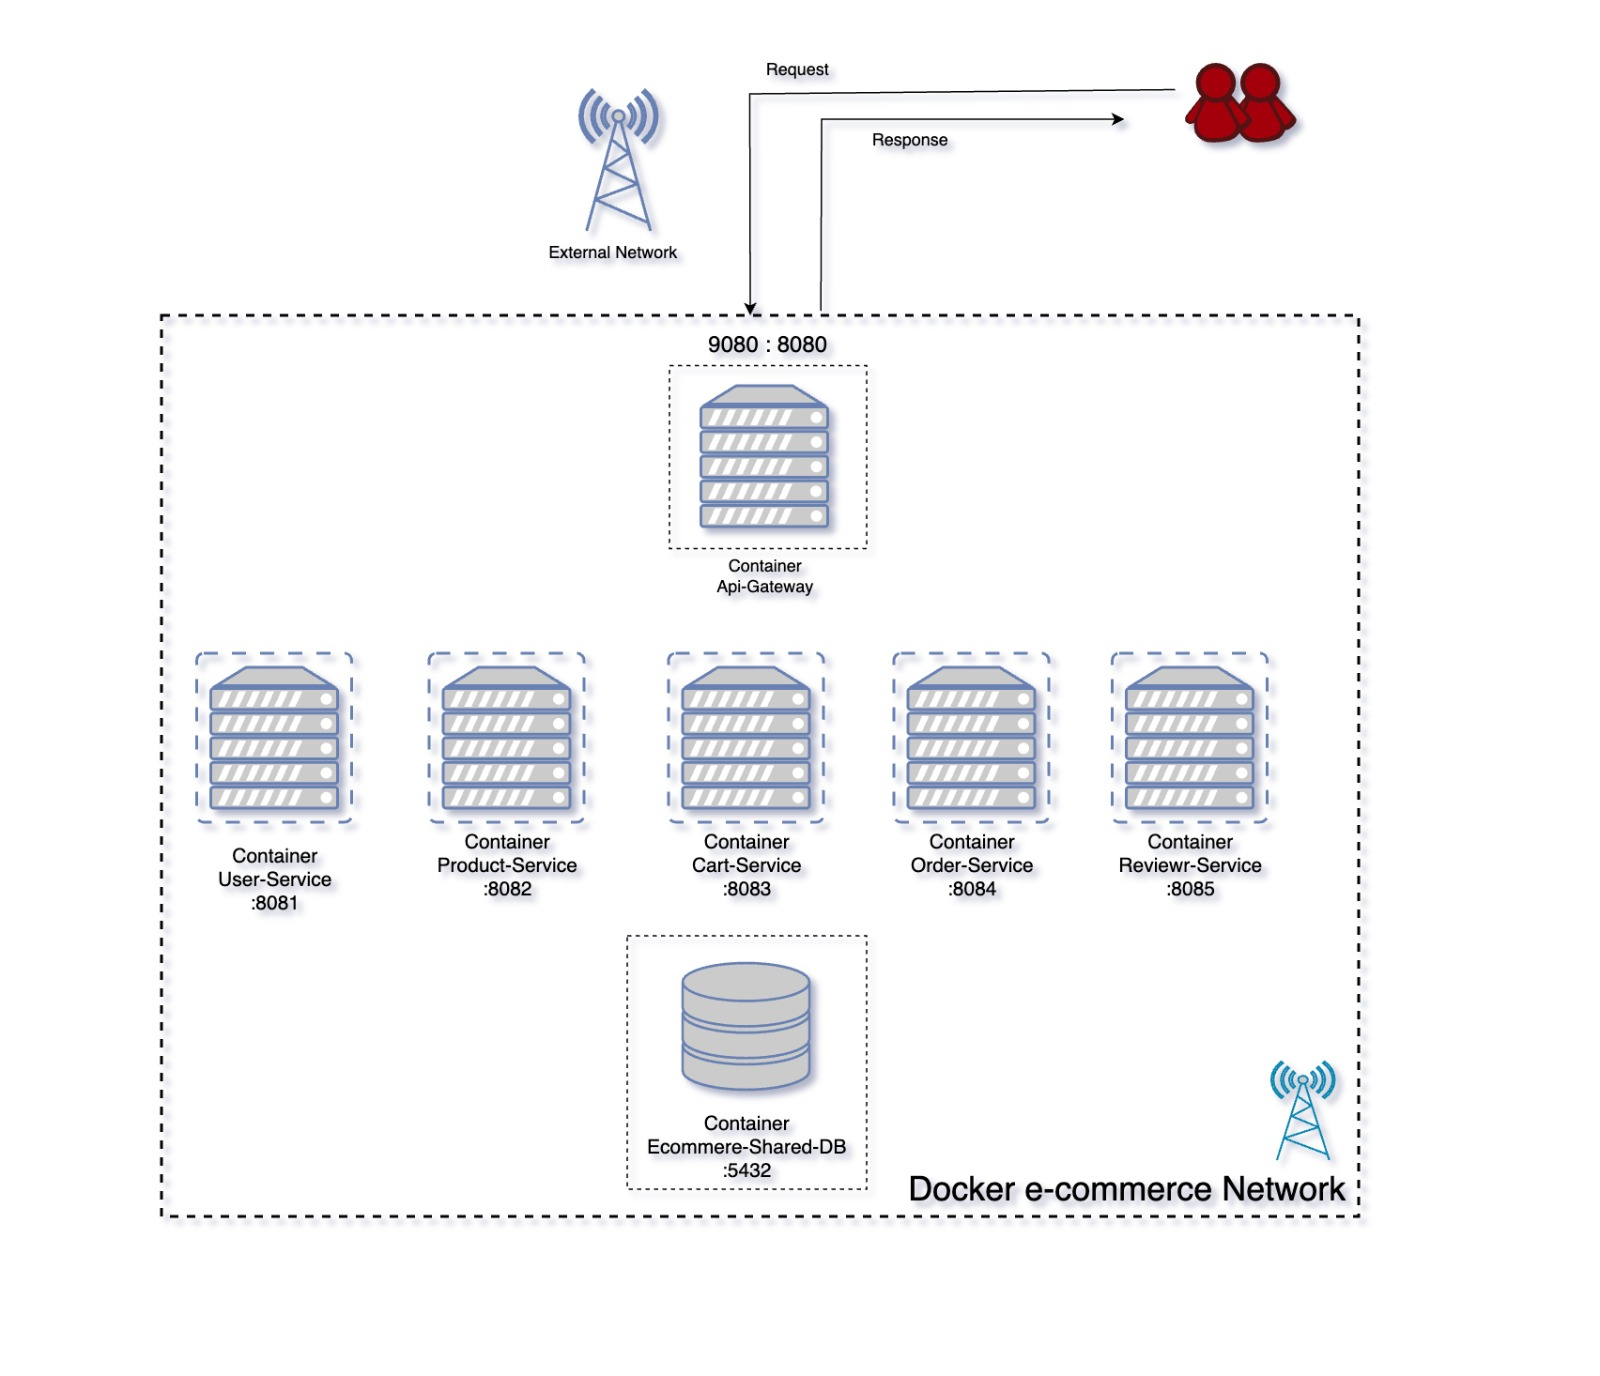
\includegraphics[width=0.95\textwidth]{images/arch-1.jpeg}
\caption{Architecture microservices de la plateforme e-commerce}
\label{fig:architecture-overview}
\end{figure}

La figure~\ref{fig:architecture-overview} illustre le flux de communication : les requêtes externes (External Network) arrivent à l'\textbf{API Gateway} (port 9080:8080) qui route vers les services backend appropriés. Chaque service communique avec la base de données partagée (\textbf{Ecommerce-Shared-DB}, port 5432) et expose ses propres APIs sur des ports dédiés :

\begin{itemize}
    \item \textbf{User-Service} (8081) : Gestion des utilisateurs et adresses
    \item \textbf{Product-Service} (8082) : Catalogue produits et catégories
    \item \textbf{Cart-Service} (8083) : Paniers d'achat utilisateur
    \item \textbf{Order-Service} (8084) : Commandes et leur cycle de vie
    \item \textbf{Review-Service} (8085) : Avis et évaluations produits
\end{itemize}

Tous les conteneurs appartiennent au réseau \texttt{Docker e-commerce Network}, permettant la résolution DNS automatique entre services.

\section{Points critiques pour le chaos engineering}

Cette architecture présente plusieurs caractéristiques qui en font une cible idéale pour les expérimentations de résilience :

\subsection{Single Point of Failure (SPOF)}

Chaque microservice est déployé en \textbf{instance unique} (pas de réplication), créant des SPOF potentiels. La défaillance d'un seul conteneur entraîne l'indisponibilité totale du service concerné.

\subsection{Dépendances inter-services}

Les services communiquent en mode \textbf{synchrone} via HTTP/REST (RestTemplate), sans mécanismes de résilience natifs :
\begin{itemize}
    \item Cart-Service dépend de User-Service et Product-Service
    \item Order-Service dépend de User-Service et Product-Service
    \item Review-Service dépend de User-Service et Product-Service
\end{itemize}

Une panne en cascade est donc possible : si Product-Service tombe, Cart-Service, Order-Service et Review-Service deviennent partiellement ou totalement inutilisables.

\subsection{Base de données partagée}

La base PostgreSQL représente un \textbf{SPOF critique} : tous les services y accèdent directement. Une défaillance ou une saturation de la base impacte l'ensemble du système.

\subsection{Réseau Docker bridge}

Le réseau \texttt{ecommerce-network} introduit une latence réseau variable et est susceptible aux perturbations (perte de paquets, délais, partitionnement réseau).

\section{Infrastructure d'observabilité}

Pour mesurer l'impact des fautes injectées, une stack complète de monitoring a été intégrée :

\subsection{Composants de monitoring}

\begin{itemize}
    \item \textbf{Prometheus} (port 9091) : Collecte des métriques en time-series avec scraping toutes les 15 secondes
    \item \textbf{Grafana} (port 3000) : Dashboards de visualisation et alerting
    \item \textbf{cAdvisor} (port 9092) : Métriques des conteneurs Docker (CPU, mémoire, réseau, I/O)
\end{itemize}

Cette infrastructure permettra de mesurer précisément l'impact des fautes : dégradation de latence, augmentation du taux d'erreurs, chute du débit, indisponibilité des services.

\section{Déploiement avec Docker Compose}

\subsection{Configuration de base}

Le fichier \texttt{docker-compose.yml} orchestre l'ensemble de l'infrastructure :

\begin{lstlisting}[language=YAML, caption={docker-compose.yml - Services principaux (extrait)}]
services:
  shared-postgres:
    image: postgres:15-alpine
    container_name: ecommerce-shared-postgres
    ports: ["5432:5432"]
    networks:
      - ecommerce-network

  user-service:
    build: ./user-service
    container_name: user-service
    ports: ["9081:8081"]
    depends_on: [shared-postgres]
    networks:
      - ecommerce-network

  product-service:
    build: ./product-service
    container_name: product-service
    ports: ["9082:8082"]
    depends_on: [shared-postgres]
    networks:
      - ecommerce-network

  # Cart, Order, Review services (similaire)
  
  api-gateway:
    build: ./api-gateway
    container_name: api-gateway
    ports: ["9080:8080"]
    environment:
      - SPRING_PROFILES_ACTIVE=docker
    depends_on:
      - user-service
      - product-service
      - cart-service
      - order-service
      - review-service
    networks:
      - ecommerce-network

networks:
  ecommerce-network:
    driver: bridge
\end{lstlisting}

\subsection{Configuration du monitoring}

\begin{lstlisting}[language=YAML, caption={docker-compose.yml - Stack d'observabilité (extrait)}]
  prometheus:
    image: prom/prometheus:latest
    container_name: prometheus
    ports: ["9091:9090"]
    volumes:
      - ./monitoring/prometheus.yml:/etc/prometheus/prometheus.yml
    networks:
      - ecommerce-network

  cadvisor:
    image: gcr.io/cadvisor/cadvisor:v0.47.0
    container_name: cadvisor
    ports: ["9092:8092"]
    volumes:
      - /:/rootfs:ro
      - /var/run:/var/run:ro
      - /sys:/sys:ro
      - /var/lib/docker/:/var/lib/docker:ro
    privileged: true
    command:
      - '--port=8092'
    networks:
      - ecommerce-network

  grafana:
    image: grafana/grafana:latest
    container_name: grafana
    ports: ["3000:3000"]
    environment:
      - GF_SECURITY_ADMIN_PASSWORD=admin
    networks:
      - ecommerce-network
\end{lstlisting}

\subsection{Configuration Prometheus}

\begin{lstlisting}[language=YAML, caption={monitoring/prometheus.yml - Cibles de scraping}]
global:
  scrape_interval: 15s

scrape_configs:
  # Métriques applicatives Spring Boot
  - job_name: 'spring-boot-apps'
    metrics_path: '/actuator/prometheus'
    static_configs:
      - targets:
          - 'user-service:8081'
          - 'product-service:8082'
          - 'cart-service:8083'
          - 'order-service:8084'
          - 'review-service:8085'
          - 'api-gateway:8080'

  # Métriques des conteneurs
  - job_name: 'cadvisor'
    static_configs:
      - targets: ['cadvisor:8092']
\end{lstlisting}

\section{Commandes de déploiement}

\begin{lstlisting}[caption={Démarrage de l'infrastructure complète}]
# Construction et démarrage de tous les services
docker compose up --build -d

# Vérification de l'état des conteneurs
docker compose ps

# Consultation des logs d'un service
docker compose logs -f product-service

# Arrêt et nettoyage complet
docker compose down -v
\end{lstlisting}

\subsection{Accès aux interfaces}

\begin{table}[H]
\centering
\begin{tabular}{ll}
\toprule
\textbf{Interface} & \textbf{URL} \\
\midrule
API Gateway & \texttt{http://localhost:9080} \\
Grafana & \texttt{http://localhost:3000} (admin/admin) \\
Prometheus & \texttt{http://localhost:9091} \\
cAdvisor & \texttt{http://localhost:9092} \\
Product Service (direct) & \texttt{http://localhost:9082} \\
\bottomrule
\end{tabular}
\caption{Points d'accès de l'infrastructure}
\end{table}

\section*{Conclusion du chapitre}

Ce chapitre a présenté l'architecture cible de nos expérimentations de chaos engineering : une plateforme e-commerce microservices avec cinq services métiers, une API Gateway et une base PostgreSQL partagée. 

Les caractéristiques clés identifiées sont :
\begin{itemize}
    \item \textbf{Instances uniques} : chaque service est un SPOF potentiel
    \item \textbf{Dépendances synchrones} : risque de pannes en cascade
    \item \textbf{Base partagée} : SPOF critique de données
    \item \textbf{Aucun mécanisme de résilience} : pas de retry, circuit breaker, timeout configuré
\end{itemize}

L'infrastructure de monitoring (Prometheus, Grafana, cAdvisor) est en place pour mesurer précisément l'impact des fautes qui seront injectées.

Dans le chapitre 2, nous présenterons les scénarios de test de charge et les protocoles d'injection de fautes qui seront appliqués sur cette architecture, en combinant JMeter pour générer la charge et Pumba pour injecter les pannes.

% =====================================================
% CHAPITRE 2 : TESTS DE CHARGE ET INJECTION DE FAUTES
% =====================================================
\chapter{Tests de Charge et Injection de Fautes}
\label{chap:tests-chaos}

\section{Introduction}

Ce chapitre présente la méthodologie expérimentale complète de nos tests de chaos engineering. Nous combinons deux approches complémentaires : la génération de charge réaliste avec \textbf{Apache JMeter} pour simuler des utilisateurs réels, et l'injection de fautes contrôlées avec \textbf{Pumba} pour provoquer des défaillances ciblées sur l'infrastructure.

L'objectif est de mesurer la résilience du système sous conditions normales puis dégradées, en observant les métriques de performance (latence, débit, taux d'erreurs) et de disponibilité via les dashboards Grafana configurés au chapitre précédent.

\section{Tests de charge avec Apache JMeter}

\subsection{Présentation de JMeter}

Apache JMeter est un outil open-source de test de performance permettant de simuler des charges utilisateur sur des applications web. Il offre :
\begin{itemize}
    \item Simulation de multiples utilisateurs concurrents
    \item Support de protocoles variés (HTTP, HTTPS, REST, SOAP)
    \item Extraction et validation de données (JSON, XML)
    \item Génération de rapports de performance détaillés
    \item Scripting avec variables, boucles et conditions
\end{itemize}

\subsection{Scénarios de test développés}

Trois scénarios JMeter ont été développés pour couvrir différents niveaux de complexité et de charge :

\subsubsection{Test 1 : User Service Load Test}

\textbf{Objectif} : Valider la capacité du User Service à gérer des opérations de création d'utilisateurs et d'adresses sous charge modérée.

\textbf{Configuration} :
\begin{itemize}
    \item \textbf{Nombre d'utilisateurs virtuels} : 50
    \item \textbf{Ramp-up} : 30 secondes
    \item \textbf{Itérations} : 10 par utilisateur
\end{itemize}

\textbf{Scénario} :
\begin{enumerate}
    \item \textbf{Create User} : Création d'un utilisateur avec username, email et mot de passe uniques
    \item \textbf{Extract User ID} : Extraction de l'ID utilisateur créé via JSON Extractor
    \item \textbf{Create Address} : Création d'une adresse de livraison pour cet utilisateur
    \item \textbf{Get All Users} : Récupération de la liste complète des utilisateurs
    \item \textbf{Think Time} : Pause aléatoire entre 500ms et 1500ms
\end{enumerate}

\textbf{Assertions} :
\begin{itemize}
    \item Code HTTP 201 (Created) ou 409 (Conflict si doublon) pour Create User
    \item Code HTTP 200 (OK) pour Get All Users
\end{itemize}

\subsubsection{Test 2 : Product Service Load Test}

\textbf{Objectif} : Évaluer les performances du catalogue produits sous forte charge de consultation, simulant un pic de trafic e-commerce.

\textbf{Configuration} :
\begin{itemize}
    \item \textbf{Nombre d'utilisateurs virtuels} : 100
    \item \textbf{Ramp-up} : 60 secondes
    \item \textbf{Itérations} : 20 par utilisateur
\end{itemize}

\textbf{Scénario} :
\begin{enumerate}
    \item \textbf{Get All Products} : Récupération du catalogue complet
    \item \textbf{Search Products} : Recherche avec mot-clé aléatoire parmi : laptop, phone, book, shoes, gadget
    \item \textbf{Get Products by Category} : Filtrage par catégorie (ID aléatoire 1-4)
    \item \textbf{Get Product by ID} : Consultation détaillée d'un produit (ID aléatoire 1-5)
    \item \textbf{Think Time} : Pause aléatoire entre 200ms et 1000ms
\end{enumerate}

\textbf{Points d'attention} :
\begin{itemize}
    \item Ce test génère \textbf{2000 requêtes totales} (100 users × 20 iterations)
    \item Sollicitation intensive du Product Service et de la base de données
    \item Permet d'observer la dégradation progressive sous charge
\end{itemize}

\subsubsection{Test 3 : E2E Shopping Flow}

\textbf{Objectif} : Simuler un parcours complet d'achat (end-to-end) sollicitant l'ensemble des microservices de manière coordonnée.

\textbf{Configuration} :
\begin{itemize}
    \item \textbf{Nombre d'utilisateurs virtuels} : 20
    \item \textbf{Ramp-up} : 60 secondes
    \item \textbf{Itérations} : 5 par utilisateur
\end{itemize}

\textbf{Scénario détaillé} :
\begin{enumerate}
    \item \textbf{Get Users with Addresses} : Récupération d'un utilisateur avec ses adresses
    \begin{itemize}
        \item Extraction aléatoire d'un \texttt{USER\_ID} et \texttt{ADDRESS\_ID}
    \end{itemize}
    
    \item \textbf{Browse Products} : Navigation dans le catalogue
    \begin{itemize}
        \item Extraction d'un \texttt{PRODUCT\_ID} aléatoire
    \end{itemize}
    
    \item \textbf{View Product Details} : Consultation détaillée du produit sélectionné
    
    \item \textbf{Add to Cart (Loop 3×)} : Ajout de 3 produits au panier
    
    \item \textbf{View Cart} : Consultation du panier complet
    
    \item \textbf{Create Order} : Transformation du panier en commande
    \begin{itemize}
        \item Extraction de l'\texttt{ORDER\_ID} généré
    \end{itemize}
    
    \item \textbf{View Order Details} : Consultation de la commande créée
    
    \item \textbf{Think Time} : Pause aléatoire entre 1s et 3s
\end{enumerate}

Ce scénario E2E est particulièrement sensible aux pannes, car il sollicite l'ensemble des services de manière séquentielle.



\section{Injection de fautes avec Pumba}

\subsection{Présentation de Pumba}

\begin{figure}[H]
\centering
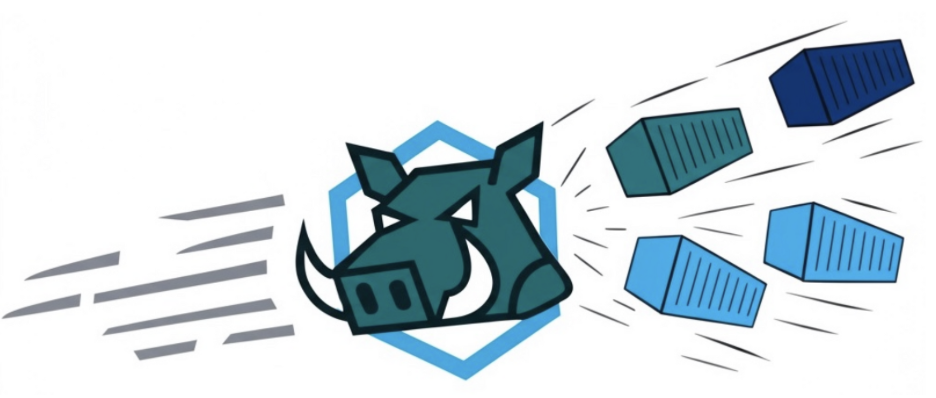
\includegraphics[width=0.6\textwidth]{images/Pumba.png}
\caption{Pumba}
\end{figure}

Pumba est un outil de chaos engineering spécialisé pour Docker, permettant d'injecter des fautes au niveau conteneur et réseau. Il s'interface directement avec l'API Docker pour manipuler les conteneurs en cours d'exécution.

\textbf{Capacités principales} :
\begin{itemize}
    \item \textbf{Stop/Kill} : Arrêt gracieux ou brutal de conteneurs
    \item \textbf{Pause/Unpause} : Gel temporaire d'un conteneur
    \item \textbf{Network Emulation (netem)} : Latence, perte de paquets, duplication, corruption
    \item \textbf{Stress} : Surcharge CPU/mémoire
\end{itemize}

\subsection{Configuration de l'environnement de test}

\subsubsection{Contexte et contraintes}

\begin{itemize}
    \item \textbf{Point d'entrée unique} : Spring Cloud Gateway 
    \item \textbf{Instances uniques} : Chaque service déployé en 1 seule réplica
    \item \textbf{Pas de politique de redémarrage} : \texttt{restart} non défini dans docker-compose.yml
    \item \textbf{Conséquence} : Une panne de conteneur = indisponibilité totale du service (SPOF)
\end{itemize}

\subsubsection{Cible des tests}

\begin{itemize}
    \item \textbf{Service cible} : \texttt{product-service}
    \item \textbf{Raison du choix} : Service le plus sollicité par les scénarios JMeter
    \item \textbf{Sélection Pumba} : Regex exacte \texttt{re2:\^{}product-service\$}
    \item \textbf{Réseau} : \texttt{ecommerce-network} (bridge)
    \item \textbf{Image TC} : \texttt{gaiadocker/iproute2} pour les règles \texttt{netem}
\end{itemize}

\subsection{Scénarios de pannes}

\subsubsection{Scénario 1 : Arrêt temporaire (Stop)}

\textbf{Objectif} : Simuler une maintenance planifiée ou un redémarrage gracieux du service.

\begin{lstlisting}[caption={Commande Pumba - Stop 30s}]
docker run -it --rm \
  -v /var/run/docker.sock:/var/run/docker.sock \
  --network ecommerce-network \
  gaiaadm/pumba:0.9.0 \
  stop --duration 30s --time 10s re2:^product-service$
\end{lstlisting}

\textbf{Paramètres} :
\begin{itemize}
    \item \texttt{--duration 30s} : Le conteneur reste arrêté pendant 30 secondes
    \item \texttt{--time 10s} : Délai avant l'injection (permet de démarrer JMeter d'abord)
\end{itemize}

\textbf{Comportement attendu} :
\begin{itemize}
    \item $t = 10s$ : Arrêt gracieux du conteneur (\texttt{SIGTERM})
    \item $t = 10s \rightarrow 40s$ : Product Service indisponible (30s downtime)
    \item $t = 40s$ : Redémarrage automatique du conteneur
    \item Disponibilité théorique : $\frac{270s}{300s} \times 100 = 90\%$ (sur fenêtre 5 min)
\end{itemize}

\textbf{Impact observé} :
\begin{itemize}
    \item Requêtes vers Product Service → erreurs 502/503/504 (Bad Gateway/Service Unavailable/Timeout)
    \item Services dépendants (Cart, Order, Review) → erreurs partielles ou complètes
    \item Métrique Grafana \texttt{up\{instance="product-service:8082"\}} → passe de 1 à 0 puis retour à 1
\end{itemize}

\subsubsection{Scénario 2 : Crash brutal (Kill)}

\textbf{Objectif} : Simuler un crash applicatif ou système (OOM, segfault, kernel panic).

\begin{lstlisting}[caption={Commande Pumba - Kill SIGTERM}]
docker run -it --rm \
  -v /var/run/docker.sock:/var/run/docker.sock \
  gaiaadm/pumba:0.9.0 \
  kill --signal SIGTERM re2:^product-service$
\end{lstlisting}

\begin{lstlisting}[caption={Commande Pumba - Kill SIGKILL (brutal)}]
docker run -it --rm \
  -v /var/run/docker.sock:/var/run/docker.sock \
  gaiaadm/pumba:0.9.0 \
  kill --signal SIGKILL re2:^product-service$
\end{lstlisting}

\textbf{Différence SIGTERM vs SIGKILL} :
\begin{itemize}
    \item \textbf{SIGTERM} : Signal gracieux, permet au processus de nettoyer les ressources (fermer connexions DB, flush logs)
    \item \textbf{SIGKILL} : Terminaison immédiate, aucun cleanup possible (simule un kill -9 ou perte d'alimentation)
\end{itemize}

\textbf{Comportement observé} :
\begin{itemize}
    \item Sans \texttt{restart: always} → Le conteneur reste DOWN indéfiniment
    \item Product Service indisponible jusqu'à intervention manuelle (\texttt{docker compose up -d})
    \item Disponibilité = 0\% après le kill
\end{itemize}

\subsubsection{Scénario 3 : Latence réseau (Netem Delay)}

\textbf{Objectif} : Simuler une dégradation réseau (congestion, distance géographique, routage sous-optimal).

\begin{lstlisting}[caption={Commande Pumba - Latence 500ms ±100ms}]
docker run -it --rm \
  -v /var/run/docker.sock:/var/run/docker.sock \
  --network ecommerce-network \
  gaiaadm/pumba:0.9.0 netem \
    --tc-image gaiadocker/iproute2 \
    --duration 2m delay \
      --time 500 --jitter 100 --distribution normal \
    re2:^product-service$
\end{lstlisting}

\textbf{Paramètres netem} :
\begin{itemize}
    \item \texttt{--time 500} : Délai moyen de 500ms ajouté à chaque paquet
    \item \texttt{--jitter 100} : Variation aléatoire de ±100ms
    \item \texttt{--distribution normal} : Distribution gaussienne du jitter
    \item \texttt{--duration 2m} : Injection active pendant 2 minutes
\end{itemize}

\textbf{Résultat} : Latence effective entre 400ms et 600ms (distribution normale).

\textbf{Impact observé} :
\begin{itemize}
    \item Latence p95 des requêtes HTTP → augmentation de 50-100ms à 600-700ms
    \item Timeout potentiels si RestTemplate configuré avec timeout < 700ms
    \item Débit (throughput) → diminution de 20-40\% due aux requêtes plus lentes
    \item Disponibilité → reste à 100\% (service répond, mais lentement)
\end{itemize}

\subsubsection{Scénario 4 : Perte de paquets (Netem Loss)}

\textbf{Objectif} : Simuler une connexion réseau instable (WiFi dégradé, réseau saturé).

\begin{lstlisting}[caption={Commande Pumba - Perte 20\% de paquets}]
docker run -it --rm \
  -v /var/run/docker.sock:/var/run/docker.sock \
  --network ecommerce-network \
  gaiaadm/pumba:0.9.0 netem \
    --tc-image gaiadocker/iproute2 \
    --duration 2m loss --percent 20 \
    re2:^product-service$
\end{lstlisting}

\textbf{Paramètres} :
\begin{itemize}
    \item \texttt{--percent 20} : 20\% des paquets réseau sont aléatoirement supprimés
    \item Effet cumulatif : requête HTTP nécessite plusieurs paquets (requête + réponse)
\end{itemize}

\textbf{Impact observé} :
\begin{itemize}
    \item Requêtes HTTP → certaines échouent directement (paquets perdus)
    \item Retransmissions TCP → augmentation de la latence (exponential backoff)
    \item Taux d'erreurs → 5-15\% de requêtes en échec
    \item Latence p95 → augmentation de 100-200ms due aux retransmissions
    \item Débit → diminution de 30-50\%
    \item Disponibilité apparente → 85-95\% (certaines requêtes passent)
\end{itemize}

\subsubsection{Scénario 5 : Chaos continu (micro-coupures périodiques)}

\textbf{Objectif} : Simuler des micro-instabilités réseau répétées (flapping network).

\begin{lstlisting}[caption={Commande Pumba - Cycles de latence 15s toutes les 30s}]
docker run -it --rm \
  -v /var/run/docker.sock:/var/run/docker.sock \
  gaiaadm/pumba:0.9.0 \
  --interval 30s --random netem \
    --tc-image gaiadocker/iproute2 \
    --duration 15s delay --time 200 \
    re2:^product-service$
\end{lstlisting}

\textbf{Paramètres} :
\begin{itemize}
    \item \texttt{--interval 30s} : Nouvelle injection toutes les 30 secondes
    \item \texttt{--duration 15s} : Chaque injection dure 15 secondes
    \item \texttt{--random} : Ajoute un délai aléatoire avant chaque injection
    \item \texttt{delay --time 200} : Latence de 200ms pendant les 15s actives
\end{itemize}

\textbf{Comportement} :
\begin{itemize}
    \item Cycle : 15s de latence → 15s normal → 15s latence → ...
    \item Crée des oscillations dans les métriques (pics de latence périodiques)
\end{itemize}

\textbf{Impact observé} :
\begin{itemize}
    \item Métriques Grafana → courbes en dents de scie (oscillations)
    \item Latence p95 → pics périodiques à 250-300ms
    \item Taux d'erreurs → pics légers pendant les fenêtres de latence
    \item Disponibilité → reste proche de 100\% mais avec dégradations intermittentes
\end{itemize}

\section{Protocole expérimental}

\subsection{Méthodologie générale}

Chaque test suit un protocole en trois phases pour mesurer l'impact des fautes :

\begin{figure}[H]
\centering
\begin{tikzpicture}[scale=0.8]
\draw[->] (0,0) -- (14,0) node[right] {Temps};
\draw[->] (0,0) -- (0,4) node[above] {Métriques};

% Baseline
\draw[thick, blue] (0,3) -- (5,3) node[midway, above] {Baseline};
\draw[dashed] (5,0) -- (5,4) node[above] {$t_1$};

% Chaos
\draw[thick, red] (5,3) -- (5,1.5) -- (7,1.5) -- (7,1) -- (10,1);
\node[red, above] at (7.5,1.5) {Injection};
\draw[dashed] (10,0) -- (10,4) node[above] {$t_2$};

% Recovery
\draw[thick, green!60!black] (10,1) -- (10.5,1.5) -- (11,2) -- (14,2.8);
\node[green!60!black, above] at (12,2.5) {Recovery};

\end{tikzpicture}
\caption{Chronologie expérimentale : Baseline → Chaos → Recovery}
\end{figure}

\textbf{Phase 1 : Baseline (5 minutes)} :
\begin{itemize}
    \item Système en fonctionnement normal
    \item Exécution du test JMeter pour établir les métriques de référence
    \item Observation : latence nominale, taux d'erreurs $\approx$ 0\%, débit stable
\end{itemize}

\textbf{Phase 2 : Chaos (2-5 minutes)} :
\begin{itemize}
    \item Injection de la faute Pumba (stop/kill/delay/loss)
    \item Poursuite de l'exécution JMeter (même charge)
    \item Observation : dégradation des métriques en temps réel
\end{itemize}

\textbf{Phase 3 : Recovery (5 minutes)} :
\begin{itemize}
    \item Fin de l'injection (Pumba se termine ou conteneur redémarre)
    \item Observation du retour à la normale
    \item Mesure : temps de récupération (recovery time)
\end{itemize}

\subsection{Matrice de tests}

\begin{table}[H]
\centering
\small
\begin{tabular}{lccc}
\toprule
\textbf{Scénario Pumba} & \textbf{Test JMeter} & \textbf{Durée Chaos} & \textbf{Durée Totale} \\
\midrule
Stop 30s & Product Load & 30s & ~10 min \\
Kill SIGTERM & Product Load & Indéfini & ~8 min \\
Kill SIGKILL & E2E Shopping & Indéfini & ~15 min \\
Delay 500ms & Product Load & 2 min & ~12 min \\
Loss 20\% & Product Load & 2 min & ~12 min \\
Chaos continu & E2E Shopping & 5 min & ~20 min \\
\bottomrule
\end{tabular}
\caption{Matrice des combinaisons test JMeter × scénario Pumba}
\end{table}

\subsection{Commandes d'exécution coordonnées}

\textbf{Terminal 1 - Démarrage JMeter} :
\begin{lstlisting}[caption={Lancement test JMeter en mode non-GUI}]
# Product Service Load Test
jmeter -n -t jmeter-tests/product-service-load-test.jmx

# E2E Shopping Flow
jmeter -n -t jmeter-tests/e2e-shopping-flow.jmx
\end{lstlisting}

\textbf{Terminal 2 - Injection Pumba (après 1 minute de baseline)} :
\begin{lstlisting}[caption={Injection de faute avec timing}]
# Attendre 60s pour baseline, puis injecter
sleep 60 && docker run -it --rm \
  -v /var/run/docker.sock:/var/run/docker.sock \
  --network ecommerce-network \
  gaiaadm/pumba:0.9.0 netem \
    --tc-image gaiadocker/iproute2 \
    --duration 2m delay --time 500 --jitter 100 \
    re2:^product-service$
\end{lstlisting}

\textbf{Terminal 3 - Surveillance Grafana} :
\begin{itemize}
    \item Ouvrir le dashboard "Product Service – Application \& Container"
    \item Activer l'auto-refresh (5s ou 10s)
    \item Ajouter des annotations manuelles aux moments clés :
    \begin{itemize}
        \item Annotation "Baseline Start" à $t_0$
        \item Annotation "Chaos Injection" à $t_1$ (commande Pumba lancée)
        \item Annotation "Chaos End" à $t_2$ (fin d'injection)
    \end{itemize}
\end{itemize}

\section*{Conclusion du chapitre}

Ce chapitre a présenté la méthodologie complète de nos expérimentations de chaos engineering. Nous avons détaillé :

\begin{itemize}
    \item \textbf{Trois scénarios JMeter} : User Load (50 users), Product Load (100 users), E2E Shopping (20 users)
    \item \textbf{Cinq types de pannes Pumba} : Stop, Kill (SIGTERM/SIGKILL), Delay, Loss, Chaos continu
    \item \textbf{Protocole expérimental} : Baseline → Chaos → Recovery avec captures Grafana annot

% =====================================================
\chapter{Surveillance et Visualisation des Microservices}
\label{chap:mesures}


\section{Introduction}
Avec la montée en puissance des architectures distribuées basées sur les microservices, les organisations doivent gérer un grand nombre de services interdépendants. La supervision devient alors une nécessité afin de garantir :
\begin{itemize}
     \item Une haute disponibilité,
    \item Une résolution rapide des incidents,
    \item Une optimisation des ressources.
\end{itemize}
Ce chapitre décrit une solution pratique et standardisée pour surveiller les microservices déployés dans un environnement Docker.

\section{Architecture de la solution}

\subsection{Prometheus}
\begin{figure}[H]
\centering

\includegraphics[width=0.3\textwidth]{images/prometheus.png}
\caption{Prometheus}
\label{fig:architecture-overview}
\end{figure}

Prometheus est un \textit{système de monitoring open-source} orienté séries temporelles. Il collecte les métriques via des \textit{jobs de scraping} configurés dans un fichier \texttt{prometheus.yml}. Ces métriques sont stockées dans une base de données interne et accessibles via le langage de requête \textbf{PromQL}.

\subsection{Grafana}
\begin{figure}[H]
\centering

\includegraphics[width=0.3\textwidth]{images/grafana.jpeg}
\caption{Grafana}
\label{fig:architecture-overview}
\end{figure}
Grafana est un outil de \textit{visualisation} permettant de créer des \textit{tableaux de bord interactifs}. Il se connecte à Prometheus comme source de données et offre des représentations graphiques telles que des courbes, des jauges et des alertes personnalisées.

\subsection{Spring Boot Actuator et Micrometer}
\begin{figure}[H]
\centering

\includegraphics[width=0.5\textwidth]{images/spring_boot_actuators.jpg}
\caption{Spring Boot Actuator}
\label{fig:architecture-overview}
\end{figure}
\begin{itemize}
    \item \textbf{Actuator} expose des endpoints REST permettant de consulter l’état et les métriques des applications Spring Boot.
    \item \textbf{Micrometer} sert de pont entre Actuator et des systèmes de monitoring comme Prometheus, en standardisant l’exposition des métriques.
    \item Exemples de métriques disponibles : temps de réponse, taux d’erreurs, disponibilité, consommation mémoire.
\end{itemize}

\subsection{cAdvisor}
\begin{figure}[H]
\centering

\includegraphics[width=0.3\textwidth]{images/cadvisor.png}
\caption{cAdvisor}
\label{fig:architecture-overview}
\end{figure}
cAdvisor est un démon développé par Google pour collecter et exposer les métriques de \textbf{conteneurs Docker}. Il fournit des informations détaillées sur :
\begin{itemize}
    \item  L’utilisation CPU,
    \item  La mémoire,
    \item  Les I/O disque,
    \item  Le trafic réseau.
\end{itemize}

\subsection{Architecture du système de surveillance}
\begin{figure}[H]
\centering
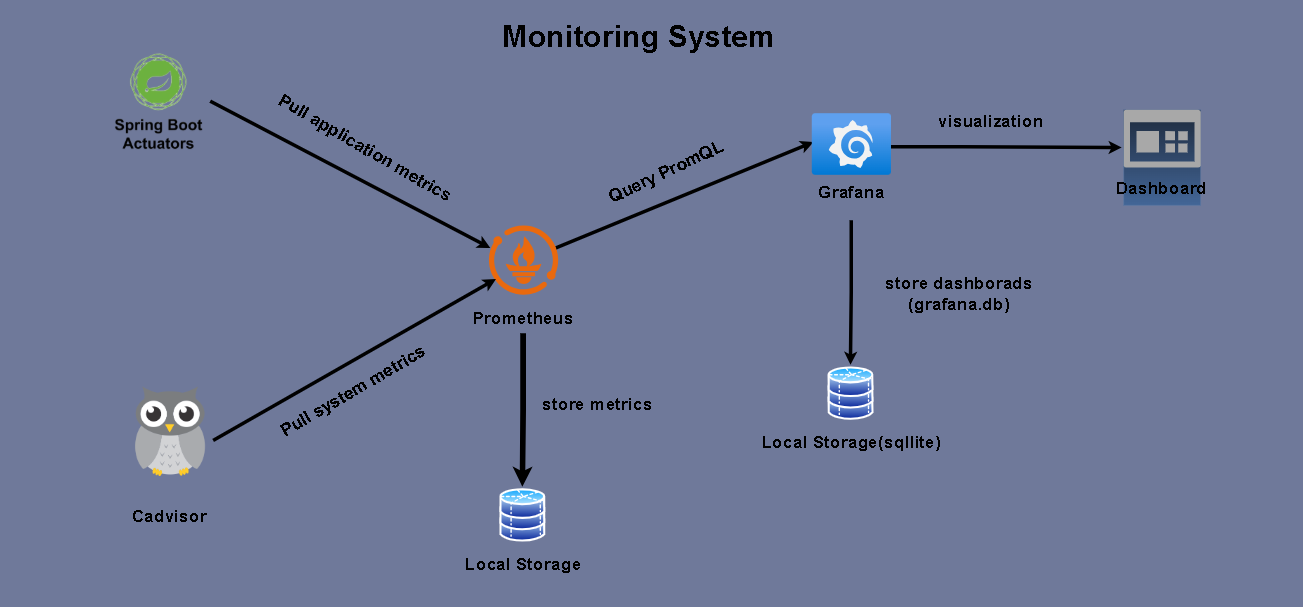
\includegraphics[width=0.95\textwidth]{images/monitoring.png}
\caption{monitoring system architecture}
\label{fig:architecture-overview}
\end{figure}

\section{Métriques surveillées}

\subsection{Côté Application (via Actuator + Micrometer)}
\begin{enumerate}
    \item  Temps de réponse (Response Time)
    \item  Taux d’erreurs (Error Rates)
    \item  Débit (Throughput - requêtes/sec)
    \item  Utilisation CPU/Mémoire par service
    \item  Disponibilité (Uptime)
    \item  Latence réseau
\end{enumerate}

\subsection{Côté Conteneurs et Système (via cAdvisor)}
\begin{enumerate}
    \item  Utilisation CPU
    \item  Consommation mémoire
    \item  Utilisation disque (I/O)
    \item  Trafic réseau (entrant/sortant)
    \item  Temps de réponse des conteneurs
    \item  Disponibilité et erreurs au niveau infrastructurel
\end{enumerate}

\section{Implémentation}

\subsection{Configuration Prometheus}
Définition des jobs pour :
\begin{itemize}
    \item Les microservices Spring Boot (\texttt{/actuator/prometheus})
    \item cAdvisor (\texttt{cadvisor:8092})
\end{itemize}
\begin{verbatim}
global:
  scrape_interval: 15s

scrape_configs:
  # Monitor Prometheus itself
  - job_name: 'prometheus'
    static_configs:
      - targets: ['prometheus:9090']

  # Monitor Spring Boot microservices
  - job_name: 'spring-boot-apps'
    metrics_path: '/actuator/prometheus'
    static_configs:
      - targets:
          - 'user-service:8081'
          - 'product-service:8082'
          - 'cart-service:8083'
          - 'order-service:8084'
          - 'review-service:8085'
          - 'api-gateway:8080'

  # Monitor cAdvisor (Docker containers)
  - job_name: 'cadvisor'
    static_configs:
      - targets: ['cadvisor:8092']
\end{verbatim}
\subsection{Déploiement Docker}
Tous les services sont déployés dans un réseau Docker commun.  
Exemple :
\begin{verbatim}
- job_name: 'spring-boot-apps'
  metrics_path: '/actuator/prometheus'
  static_configs:
    - targets: ['product-service:8082']
\end{verbatim}

\subsection{Visualisation dans Grafana}
Création de deux tableaux de bord séparés :
\begin{itemize}
    \item Application Dashboard (temps de réponse, erreurs, disponibilité, etc.)
\end{itemize}   
\begin{figure}[H]
\centering
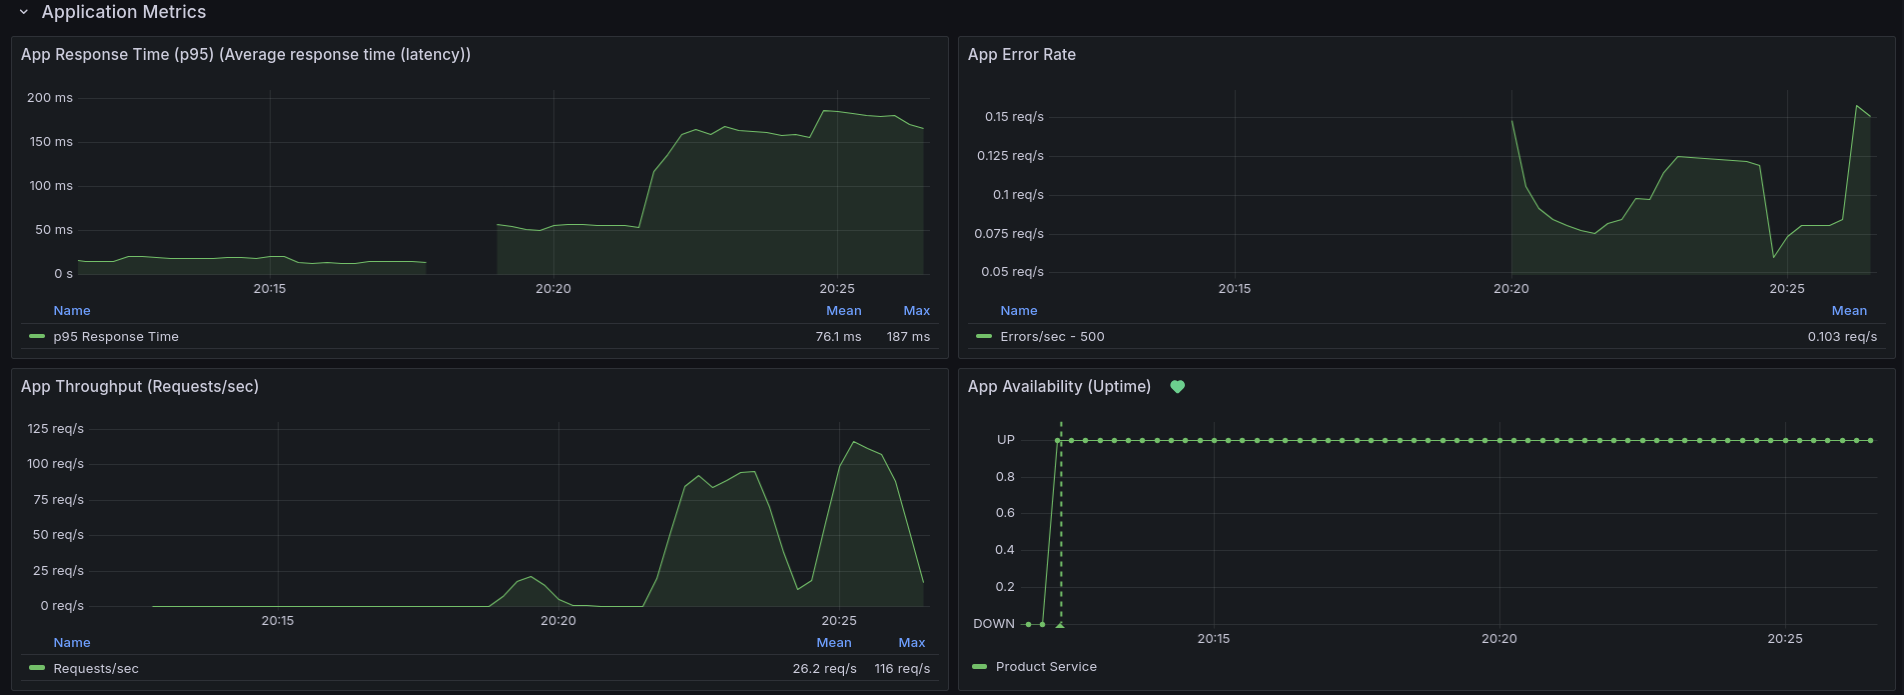
\includegraphics[width=1\textwidth]{images/app_metrics_second.png}
\caption{Dashboard des metrique au niveau d'application}
\label{fig:architecture-overview}
\end{figure}
\begin{itemize}
    \item Infrastructure Dashboard (CPU, mémoire, réseau, conteneurs).
\end{itemize}
\begin{figure}[H]
\centering
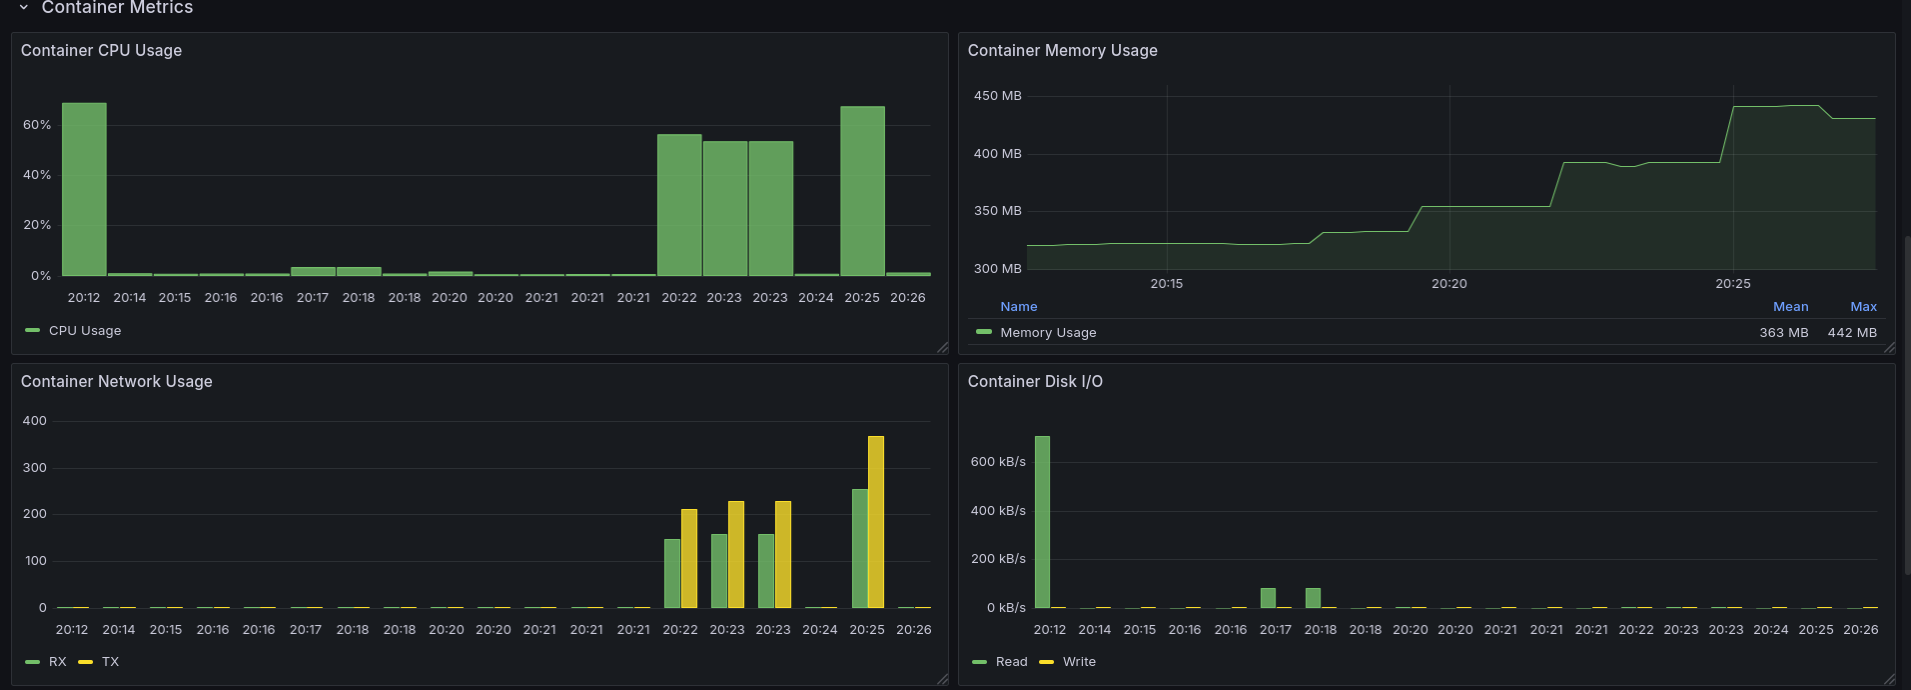
\includegraphics[width=1\textwidth]{images/container_metrics_second.png}
\caption{Dashboard des metrique au niveau de conteneur}
\label{fig:architecture-overview}
\end{figure}
\section{Résultats et Discussion}
La mise en place de ce système permet :
\begin{itemize}
    \item Une supervision unifiée des microservices et des conteneurs,
    \item Une détection proactive des anomalies grâce aux alertes configurées dans Grafana,
    \item  Une meilleure allocation des ressources en fonction des données de consommation,
    \item Une amélioration de la résilience des services grâce au suivi continu.
\end{itemize}

\section{Conclusion}
L’intégration de \textbf{Prometheus, Grafana, Actuator, Micrometer et cAdvisor} constitue une solution complète et modulaire pour la surveillance des microservices. Elle offre une visibilité à la fois applicative et infrastructurelle, ce qui permet de répondre aux enjeux de performance et de disponibilité des systèmes modernes basés sur les microservices.


% =====================================================
% CHAPITRE 3 : M E S U R E S  D ' I M P A C T
% =====================================================
\chapter{Mesurer l'impact des fautes injectées}
\label{chap:mesures}

\section{Métriques et panneaux Grafana}
\begin{itemize}
  \item \textbf{Disponibilité (Uptime)} : \texttt{up\{instance="product-service:8082"\}}.
  \item \textbf{Latence p95} : \texttt{histogram\_quantile(0.95, rate(http\_server\_requests\_seconds\_bucket[1m]))}.
  \item \textbf{Taux d'erreurs} : \texttt{rate(...\{status=~"5.."\}[1m]) / rate(...[1m])}.
  \item \textbf{Débit (Throughput)} : \texttt{sum(rate(http\_server\_requests\_seconds\_count[1m]))}.
  \item \textbf{Ressources conteneur} : CPU/RAM via cAdvisor.
\end{itemize}

\section{Synthèse attendue par scénario}
\begin{table}[H]
\centering
\begin{tabular}{lcccc}
\toprule
\textbf{Scénario} & \textbf{Uptime} & \textbf{p95} & \textbf{Erreurs} & \textbf{Throughput} \\
\midrule
Baseline & $\approx$ 100\% & 50--100 ms & $\approx$ 0\% & Stable/élevé \\
Stop 30s & $\approx$ 98.3\% (fenêtre 5min) & $\infty$ (timeouts) & 100\% (pendant 30s) & 0 puis reprise \\
Kill     & 0\% (jusqu'au restart) & N/A & $\approx$ 100\% & 0 \\
Delay 500$\pm$100ms & 100\% & 600--700 ms & 0--10\% & $\downarrow$ (20--40\%) \\
Loss 20\% & 90--95\% & 150--300 ms & 5--15\% & $\downarrow$ (20--40\%) \\
Chaos continu & $\sim$99\% & pics périodiques & pics & oscillant \\
\bottomrule
\end{tabular}
\caption{Impact des fautes (à remplacer par vos valeurs mesurées).}
\end{table}

\section{Captures et corrélation temporelle}
Nous insérons cinq captures Grafana : (i) baseline, (ii) début injection, (iii) pic d'erreurs/latence,
(iv) fin injection/début recovery, (v) retour à la normale. Les \textit{annotations} Grafana marquent les commandes Pumba.

\begin{figure}[H]
\centering
\placeholder{0.85\textwidth}{5cm}
\caption{Latence p95 pendant un \texttt{netem delay} (courbe avec pic).}
\end{figure}

\begin{figure}[H]
\centering
\placeholder{0.85\textwidth}{5cm}
\caption{Taux d'erreurs (5xx) pendant \texttt{stop}/\texttt{kill}.}
\end{figure}

\section{Discussion}
Sans réplication ni mécanismes de résilience (retry/circuit breaker), les fautes d'arrêt/kill
entraînent une indisponibilité complète du service ciblé. Les fautes réseau (\textit{delay}/\textit{loss})
conservent la disponibilité mais dégradent fortement la performance (p95 ↑, débit ↓).

\paragraph{Recommandations (priorité).}
(i) \textbf{Réplication} ($\geq$3) pour supprimer le SPOF ; 
(ii) \textbf{Resilience4j} (Retry + Circuit Breaker) côté clients ; 
(iii) \textbf{SLO + alerting} (Prometheus/Grafana) sur p95 et error rate.

% =====================================================
% CHAPITRE 4 : S T R A T E G I E S  D E  T O L E R A N C E
% =====================================================
\chapter{Stratégies de tolérance : Load Balancer et réplications}

\section{Introduction}
À la suite des différentes phases de tests de performance et de résistance menées sur notre système, plusieurs défaillances ont été constatées. En effet, lors des tests de \textit{stress} réalisés à la fois au niveau de l'infrastructure (notamment à travers la mise sous pression des conteneurs et de la latence) et au niveau applicatif (via la surcharge des services par un volume important de requêtes simultanées), le système a montré des limites notables en matière de disponibilité et de tolérance aux pannes.

Ces observations ont mis en évidence la nécessité de mettre en place une solution garantissant la continuité du service, même en cas de défaillance imprévue d'un ou plusieurs composants. L'objectif principal devient ainsi d'assurer qu'un serveur reste toujours opérationnel pour répondre aux requêtes des utilisateurs, afin d'atteindre un niveau maximal de disponibilité.

Pour répondre à cette problématique, nous avons opté pour une stratégie reposant sur la \textbf{réplication des microservices} combinée à un \textbf{mécanisme de répartition de charge} (\textit{load balancing}). Cette approche permet de distribuer intelligemment le trafic entre plusieurs instances d'un même service, tout en renforçant la résilience globale de l'architecture.


\section{Principe de la Réplication et du Load Balancing}
La mise en place d'un mécanisme de réplication et d'équilibrage de charge constitue une étape essentielle dans toute architecture microservices cherchant à garantir une haute disponibilité et une meilleure tolérance aux pannes.  

\subsection{Principe de la Réplication}
La \textbf{réplication} consiste à déployer plusieurs instances d'un même microservice afin d'assurer une continuité de service, même en cas de panne d'un conteneur ou d'une surcharge ponctuelle.  
Dans le cadre de notre projet, cette approche permet de répartir la charge de travail entre plusieurs réplicas d'un service, tout en assurant qu'au moins une instance reste disponible pour traiter les requêtes des utilisateurs.

L'intérêt principal de la réplication est donc de renforcer la \textbf{résilience du système} et d'améliorer sa \textbf{scalabilité horizontale}. En effet :
L'intérêt principal de la réplication est donc de renforcer la \textbf{résilience du système} et d'améliorer sa \textbf{scalabilité horizontale}. En effet :
\begin{itemize}
    \item Si une instance échoue, les autres peuvent immédiatement prendre le relais sans interruption du service.
    \item Le système reste \textbf{légèrement chargé} et plus \textbf{équilibré}, car l'équilibrage de charge ne s'active pas uniquement en cas de panne, mais agit en permanence pour répartir les requêtes et éviter toute surcharge localisée.
\end{itemize}

Dans notre architecture, certains services tels que le \textit{Product-Service} et le \textit{Cart-Service} ont été choisis pour être répliqués, car ils figurent parmi les plus sollicités par les requêtes des utilisateurs.  

\subsection{Principe du Load Balancing}
Afin d'exploiter pleinement les bénéfices de la réplication, il est nécessaire d'introduire un \textbf{équilibrage de charge} (\textit{load balancing}) entre les différentes instances. Ce mécanisme a pour rôle de distribuer les requêtes entrantes de manière équitable entre les réplicas d'un même service.

Le \textbf{Spring Cloud Gateway}, déjà présent dans notre architecture en tant que point d'entrée unique (\textit{API Gateway}), a été configuré pour intégrer cette logique de répartition.  
Ce dernier s'appuie sur le module \textbf{Spring Cloud LoadBalancer}, qui propose plusieurs stratégies d'équilibrage, parmi lesquelles :

\begin{itemize}
    \item \textbf{Round Robin} : distribution séquentielle des requêtes entre toutes les instances disponibles. C'est l'une des stratégies les plus simples et les plus utilisées.
    \item \textbf{Random} : sélection aléatoire d'une instance pour chaque requête, favorisant une distribution pseudo-uniforme sur la durée.
    \item \textbf{Least Connections} : la requête est envoyée à l'instance ayant actuellement le moins de connexions actives.
    \item \textbf{Weighted Response Time} : pondération des instances en fonction du temps moyen de réponse ; les plus rapides reçoivent davantage de requêtes.
    \item \textbf{Least Response Time} : sélection de l'instance la plus rapide au moment de la requête, basée sur des mesures de latence.
    \item \textbf{Availability Filtering} : les instances en surcharge ou marquées comme indisponibles sont temporairement exclues de la rotation.
    \item \textbf{Zone Avoidance} : stratégie avancée prenant en compte la répartition géographique ou zonale des instances (utile pour des déploiements multi-régions).
    \item \textbf{Consistent Hashing} : attribution déterministe d'une requête à une instance selon une clé (par exemple l'ID utilisateur), utile pour maintenir la cohérence de session.
\end{itemize}

Spring Cloud permet également la création de \textbf{stratégies personnalisées} à travers l'implémentation d'un \texttt{ReactorServiceInstanceLoadBalancer}, afin d'adapter la logique de distribution à des critères métiers spécifiques (charge CPU, métriques applicatives, affinité utilisateur, etc.).

Dans notre cas, le choix du \textit{Round Robin} s'est révélé le plus adapté à notre environnement Docker. Il offre une répartition simple, homogène et suffisante pour assurer une distribution équilibrée du trafic sans nécessiter de surveillance complexe des performances.

Ainsi, la combinaison de la \textbf{réplication} et du \textbf{load balancing} permet d'obtenir un système capable de supporter des pics de charge, de résister aux défaillances et d'assurer une meilleure expérience utilisateur.


\section{Mise en Place Technique}
Après avoir défini les principes théoriques de la réplication et du \textit{load balancing}, cette section présente la manière dont ces mécanismes ont été concrètement intégrés dans notre environnement \textbf{Docker e-commerce}.  
L'objectif est d'illustrer à la fois l'évolution de l'architecture et le fonctionnement interne du processus d'équilibrage au sein de l'API Gateway.

\subsection{Présentation de la Nouvelle Architecture Globale}
La figure~\ref{fig:replicated-architecture} illustre la nouvelle architecture adoptée après la mise en place de la réplication et du load balancing.  
Dans cette configuration, deux services critiques ont été répliqués :
\begin{itemize}
    \item \textbf{Product-Service} : déployé en deux instances (\textit{product-service-1} et \textit{product-service-2}) pour mieux répartir les requêtes liées aux produits.
    \item \textbf{Cart-Service} : également dupliqué (\textit{cart-service-1} et \textit{cart-service-2}) afin d'améliorer la gestion concurrente des paniers utilisateurs.
\end{itemize}

L'\textbf{API Gateway}, exposée sur le port \texttt{9080}, agit comme point d'entrée unique pour toutes les requêtes externes. Elle est responsable d'orienter dynamiquement les requêtes vers les réplicas disponibles, selon la stratégie d'équilibrage configurée.

\begin{figure}[H]
    \centering
    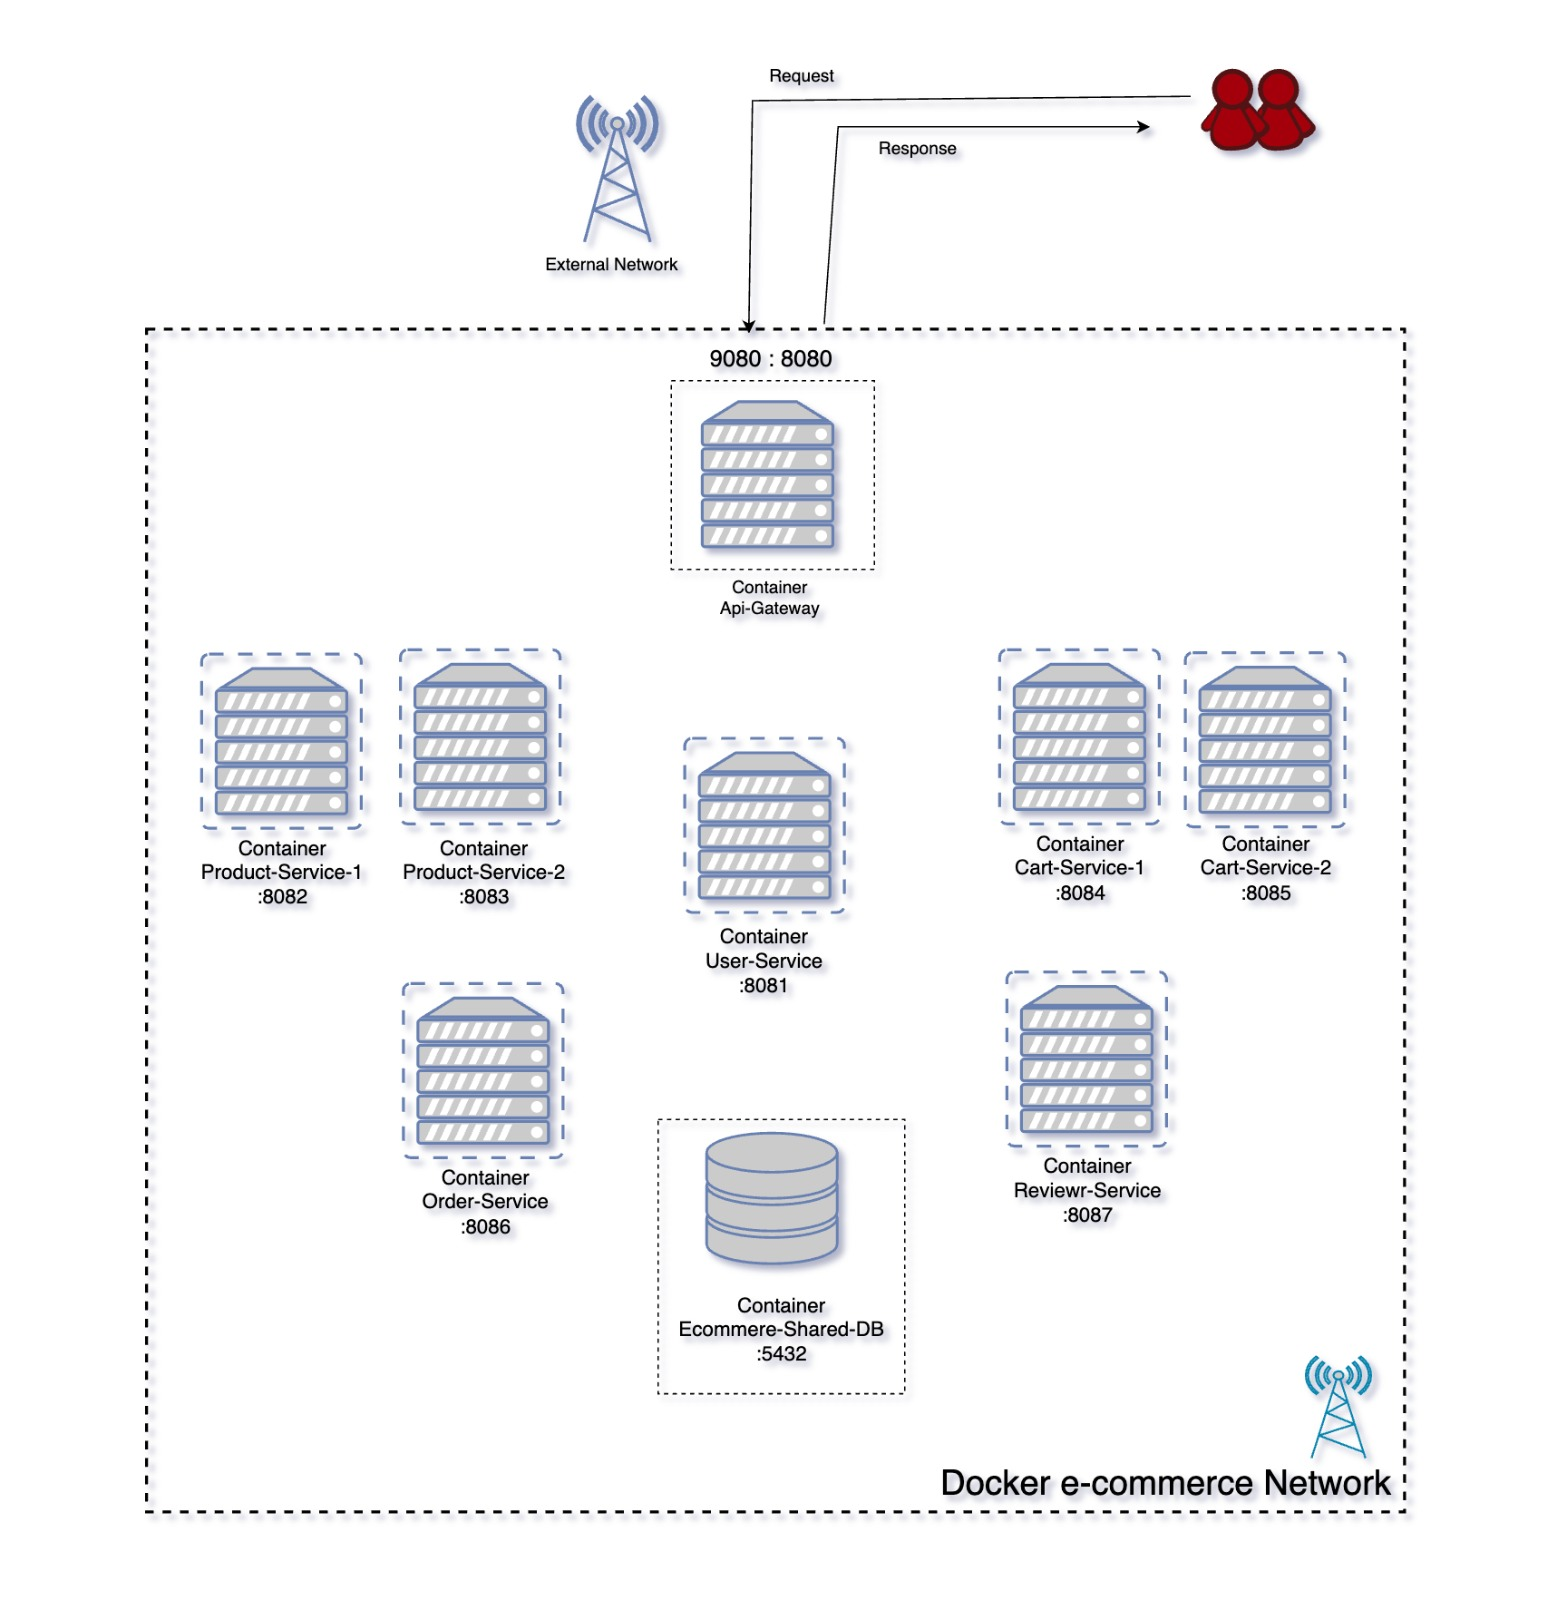
\includegraphics[width=0.95\textwidth]{images/arch-2.jpeg}
    \caption{Nouvelle architecture avec réplication et équilibrage de charge}
    \label{fig:replicated-architecture}
\end{figure}

\subsection{Fonctionnement du Processus d'Équilibrage de Charge}
Le schéma de la figure~\ref{fig:loadbalancer-flow} illustre le mécanisme interne d'équilibrage au sein de l'API Gateway.  
Lorsqu'une requête arrive depuis le réseau externe :
\begin{enumerate}
    \item Elle est d'abord reçue par l'\textbf{API Gateway}, qui agit comme point central d'accès.
    \item L'API Gateway transmet ensuite la requête au module \textbf{Spring Cloud LoadBalancer}.
    \item L'algorithme de répartition sélectionne dynamiquement l'une des instances du service ciblé (ici \textit{Product-Service-1} ou \textit{Product-Service-2}).
    \item La requête est alors acheminée vers le conteneur choisi, puis la réponse est renvoyée à l'utilisateur.
\end{enumerate}

Ce processus garantit une répartition continue du trafic, évitant toute surcharge localisée et assurant une réponse fluide et constante, même en présence de multiples utilisateurs simultanés.

\begin{figure}[H]
    \centering
    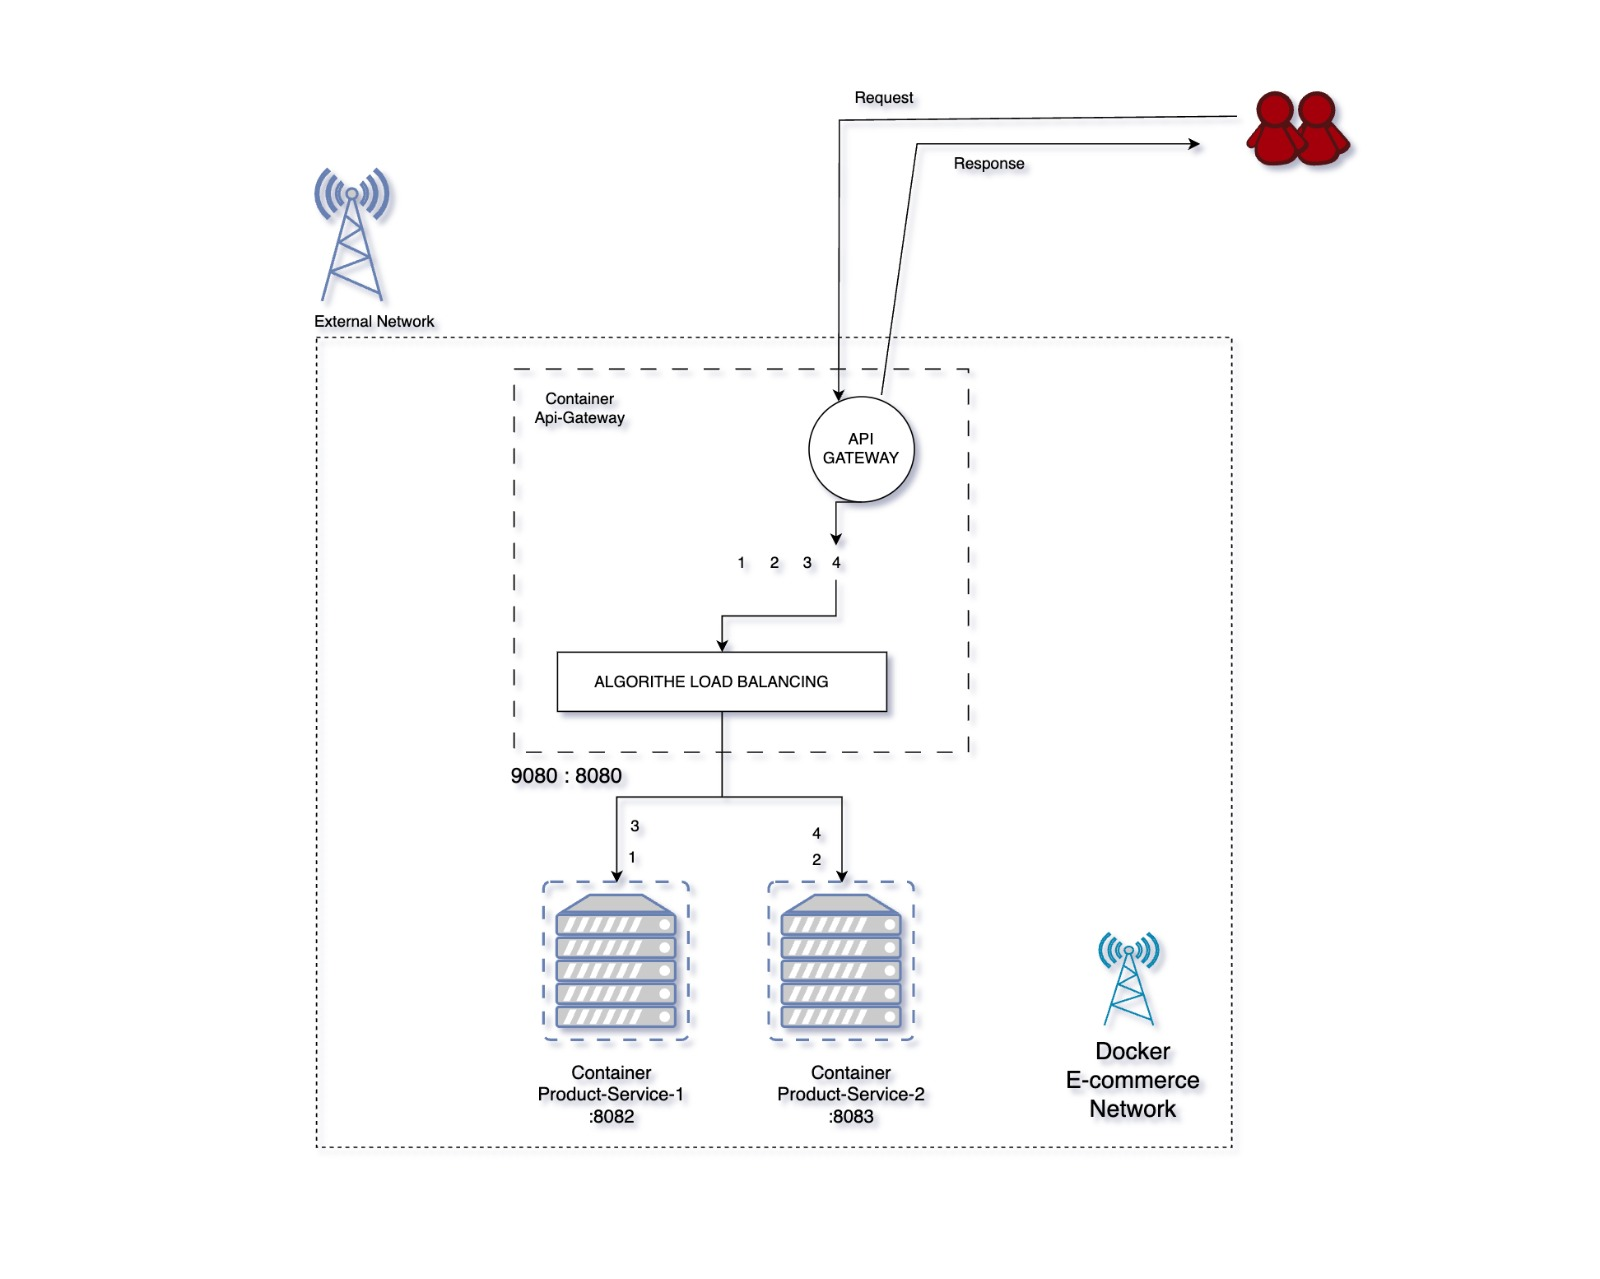
\includegraphics[width=0.85\textwidth]{images/lb-ex.jpeg}
    \caption{Mécanisme d'équilibrage des requêtes dans l'API Gateway}
    \label{fig:loadbalancer-flow}
\end{figure}

\subsection{Choix et Implémentation de la Stratégie d'Équilibrage}
La classe \texttt{LoadBalancerConfig.java} définit la stratégie de répartition utilisée par le système.  
Elle implémente un \texttt{ReactorServiceInstanceLoadBalancer}, permettant d'appliquer une logique de sélection dynamique basée sur le type d'algorithme choisi.  
Dans notre environnement, la stratégie \textbf{Round Robin} a été retenue pour sa simplicité et son efficacité, garantissant une rotation uniforme entre les réplicas.

\subsection{Résumé de l'Intégration}
En résumé, cette intégration technique a permis :
\begin{itemize}
    \item d'assurer une disponibilité constante grâce à la duplication des services critiques ;
    \item d'optimiser la répartition des requêtes via le module \texttt{Spring Cloud LoadBalancer} ;
    \item de rendre le système plus robuste et plus tolérant aux défaillances ;
    \item de préparer la plateforme aux tests de charge et scénarios de panne détaillés dans le chapitre suivant.
\end{itemize}


\section*{Conclusion du Chapitre}
Ce chapitre a permis d'introduire et de mettre en œuvre la \textbf{réplication} et le \textbf{load balancing} au sein de notre architecture microservices.  
Grâce à cette approche, le système bénéficie désormais d'une meilleure \textbf{disponibilité}, d'une \textbf{résilience accrue} et d'une \textbf{répartition équilibrée} du trafic entre les instances.

La réplication assure la continuité du service en cas de panne, tandis que le mécanisme d'équilibrage de charge, géré par \textit{Spring Cloud LoadBalancer}, répartit les requêtes de manière homogène.  
Le choix de la stratégie \textit{Round Robin} s'est montré efficace pour garantir une distribution simple et stable dans notre environnement Docker.

Cette amélioration structurelle constitue une base solide pour les \textbf{tests de performance et de résistance} présentés dans le chapitre suivant.

% =====================================================
% CONCLUSION & RECOMMANDATIONS
% =====================================================
\chapter*{Conclusion et Recommandations}
\addcontentsline{toc}{chapter}{Conclusion et Recommandations}

\textbf{Bilan.}
Les expériences montrent que, dans une topologie à \textit{instance unique}, certaines fautes (\texttt{kill} sans restart) provoquent une indisponibilité totale (\textit{SPOF}), tandis que les fautes réseau (\texttt{delay}/\texttt{loss}) dégradent fortement la \textit{latence p95} et le \textit{throughput} sous charge continue. 
Le protocole \textit{Baseline → Chaos → Recovery} et l'instrumentation Prometheus/Grafana permettent de quantifier précisément ces effets et d'objectiver les temps de récupération.

\textbf{Améliorations implémentées.}
La \textbf{réplication} des services critiques couplée à un \textbf{équilibrage de charge} (Spring Cloud LoadBalancer) atténue l'impact des pannes unitaires et lisse la performance. 
Combinée à des garde-fous applicatifs (timeouts, retries avec backoff, circuit breakers, \textit{bulkheads}), cette approche stabilise les \textit{SLI} observés.

\textbf{Recommandations opérationnelles.}
\begin{itemize}
  \item \textbf{Disponibilité \& redémarrage}: définir des politiques \texttt{restart: always/on-failure}, sondes \texttt{healthcheck}, et \texttt{readiness/liveness} (si orchestrateur K8s).
  \item \textbf{Résilience applicative}: fixer des \textit{timeouts} cohérents bout-en-bout, activer \textit{retries} bornés, \textit{circuit breakers} et \textit{bulkheads}; gérer l'\textit{idempotence} des opérations.
  \item \textbf{Topologie}: répliquer les services à fort trafic (ex. \textit{product-service}) et isoler les dépendances sensibles (DB, cache) avec limites de connexion et \textit{pooling} maîtrisé.
  \item \textbf{Observabilité}: définir des \textbf{SLO} (p95, erreurs, disponibilité), des alertes (seuils p95, saturation CPU/mémoire, erreurs 5xx) et des \textit{dashboards} orientés parcours métier.
  \item \textbf{Chaos continu}: intégrer des \textit{game days} et tests Pumba réguliers (scénarios \texttt{stop/kill/netem}), idéalement \textit{shift-left} (en pré-prod) et \textit{canary} en prod.
  \item \textbf{Capacité \& coût}: utiliser l’\textit{auto-scaling} sur métriques (CPU, RPS, p95), surveiller le coût des replicas et la contention des ressources partagées.
\end{itemize}

\textbf{Perspectives.}
Passer à un orchestrateur (Kubernetes) pour des stratégies natives (HPA, PodDisruptionBudget, PodAntiAffinity), introduire un \textbf{service mesh} (observabilité L7, \textit{retries}/\textit{timeouts} centralisés) et tester des fautes \textit{stateful} (DB failover, \textit{network partition}) afin d'élargir le périmètre de résilience.


\end{document}
